% Created 2018-04-26 周四 13:52
\documentclass[11pt]{article}
\usepackage[utf8]{inputenc}
\usepackage[T1]{fontenc}
\usepackage{fixltx2e}
\usepackage{graphicx}
\usepackage{longtable}
\usepackage{float}
\usepackage{wrapfig}
\usepackage{rotating}
\usepackage[normalem]{ulem}
\usepackage{amsmath}
\usepackage{textcomp}
\usepackage{marvosym}
\usepackage{wasysym}
\usepackage{amssymb}
\usepackage{hyperref}
\tolerance=1000
\usepackage{amsmath}
\usepackage{tikz}
\usepackage{pgfplots}
\usetikzlibrary{shapes,snakes,calc}
\date{\today}
\title{CourseraDeepLearning}
\hypersetup{
  pdfkeywords={},
  pdfsubject={},
  pdfcreator={Emacs 25.2.1 (Org mode 8.2.10)}}
\begin{document}

\maketitle
\tableofcontents

\%\#+header: :file (by-backend (html "tree.svg") (t 'nil))
\%\#+header: :imagemagick
\section{week1}
\label{sec-1}
\subsection{logistic regression}
\label{sec-1-1}
the output of y in supervised learning problem are either zero or 1
\begin{itemize}
\item given $x\in\mathbb{R}^{n_x}$, want $\hat{y}=p(y=1\mid x)$,parameters $w\in\mathbb{R}^{n_x},b\in\mathbb{r}$
output $\hat{y}=\sigma(w^tx+b)$,$\sigma(z)=\frac{1}{1+e^{-z}}$.
training example:$\{(x^{(1)},y^{(1)}),\dots,(x^{(m)},y^{(m)})\}$, want$\hat{y}^{(i)}\approx y^{(i)}$
\begin{description}
\item[{loss function}] measure how good $\hat{y}$ is when the true label is y
$\boldsymbol{l}(\hat{y},y)=-(y\text{log}\hat{y}+(1-y)\text{log}(1-\hat{y}))$
if y = 1, $\boldsymbol{l}=-\text{log}\hat{y}$, want $\hat{y}$ large
if y = 0, $\boldsymbol{l}=-\text{log}(1-\hat{y})$,want $\hat{y}$ small
\item[{cost function}] entire training set
measures how well we're doing an entire training set
$j(w,b)=\frac{1}{m}\displaystyle\sum_{i=1}^m\boldsymbol{l}(\hat{y}^{(i)},y^{(i)})$
\end{description}
\end{itemize}
\subsection{gradient descent}
\label{sec-1-2}
\begin{itemize}
\item want to find $w,b$ that minimize $j(w,b)$
\item $w:=w-\alpha\frac{\partial j(w,b)}{\partial w}$
\end{itemize}
\subsection{logistic regression gradient descent}
\label{sec-1-3}
\begin{align*}
&\frac{\partial\boldsymbol{l}(a,y)}{\partial a}=-\frac{y}{a}+\frac{1-y}{1-a}\\
&\frac{\partial a}{\partial z}=\frac{-e^{-x}}{(1+e^{-x})^2}=a(1-a)\\
&\frac{\partial\boldsymbol{l}(a,y)}{\partial z}=a(1-a)(-\frac{y}{a}+\frac{1-y}{1-a})=a-y
\end{align*}
\subsection{vectorization}
\label{sec-1-4}
\begin{description}
\item[{simd}] single instantion multiple data
\end{description}
\section{week2}
\label{sec-2}
\subsection{neural network representaion}
\label{sec-2-1}
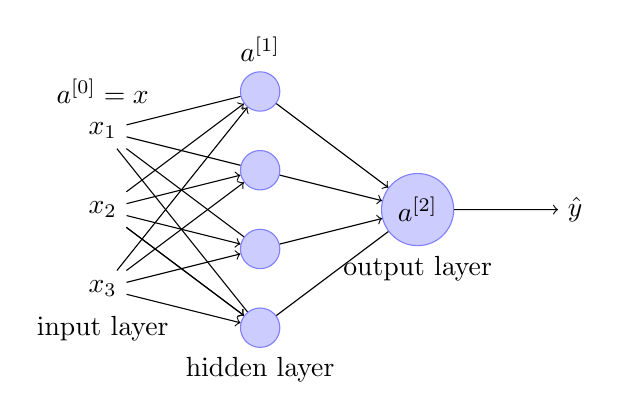
\begin{tikzpicture}
[place/.style={circle,draw=blue!50,fill=blue!20,minimum size=5mm}]
\node (x1) at (0,2.5) [label=above:{$a^{[0]}= x$}] {$x_1$};
\node (x2) at (0,1.5) {$x_2$};
\node (x3) at (0,0.5) [label=below:input layer] {$x_3$};
\node (p1) at (2,0) [place,label=below:hidden layer] {};
\node (p2) at (2,1) [place] {};
\node (p3) at (2,2) [place] {};
\node (p4) at (2,3) [place,label=above:{$a^{[1]}$}] {};
\node (c) at (4,1.5) [place,label=below:output layer] {$a^{[2]}$};
\node (y) at (6,1.5) {$\hat{y}$};
\draw [->] (x1) -- (p1) -- (c) -- (y);
\draw [->] (x1) -- (p2) -- (c);
\draw [->] (x1) -- (p4) -- (c);
\draw [->] (x2) -- (p1);
\draw [->] (x1) -- (p3) -- (c);
\draw [->] (x2) -- (p1);
\draw [->] (x2) -- (p2);
\draw [->] (x2) -- (p3);
\draw [->] (x3) -- (p3);
\draw [->] (x3) -- (p2);
\draw [->] (x3) -- (p1);
\draw [->] (x3) -- (p4);
\draw [->] (x2) -- (p4);
\end{tikzpicture}
\begin{itemize}
\item 2 layer nn
\end{itemize}
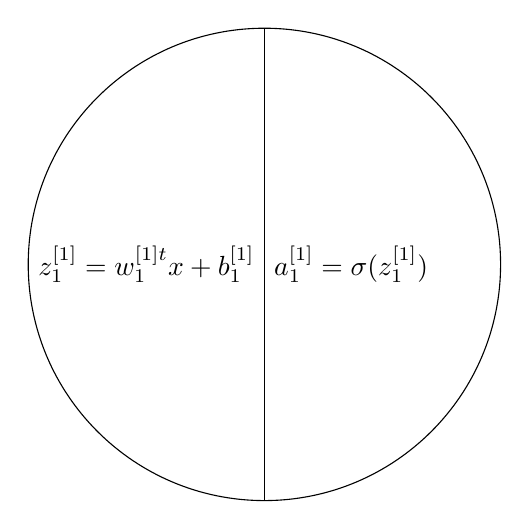
\begin{tikzpicture}
\node [circle split, draw, rotate=90] (z) {\rotatebox{-90}{$z_1^{[1]}=w_1^{[1]t}x+b_1^{[1]}$}
\nodepart{lower} \rotatebox{-90}{$a_1^{[1]}=\sigma(z_1^{[1]})$}};
\end{tikzpicture}
\begin{align*}
&z_1^{[1]}=w_1^{[1]t}x+b_1^{[1]}\quad a_1^{[1]}=\sigma(z_1^{[1]})\\
&z_2^{[1]}=w_2^{[1]t}x+b_2^{[1]}\quad a_2^{[1]}=\sigma(z_2^{[1]})\\
&z_3^{[1]}=w_3^{[1]t}x+b_3^{[1]}\quad a_3^{[1]}=\sigma(z_3^{[1]})\\
&z_4^{[1]}=w_4^{[1]t}x+b_4^{[1]}\quad a_4^{[1]}=\sigma(z_4^{[1]})\\
&z^{[2]}=w^{[2]t}a^{[1]}+b^{[2]}\quad a^{[2]}=\sigma(z^{[2]})\\
\end{align*}
\begin{pmatrix}
\mid & \mid & \cdots & \mid \\
x^{(1)} & x^{(2)} & \cdots & x^{(n)}\\
\mid & \mid & \cdots & \mid \\
\end{pmatrix}
\subsection{Activation function}
\label{sec-2-2}
\begin{itemize}
\item sigmoid function
\item hypobolic tangent function
\begin{equation*}
g(z)=\frac{e^z-e^{-z}}{e^z+e^{-z}}
\end{equation*}
\begin{equation*}
g'(z)=1-(tanh(z))^2
\end{equation*}
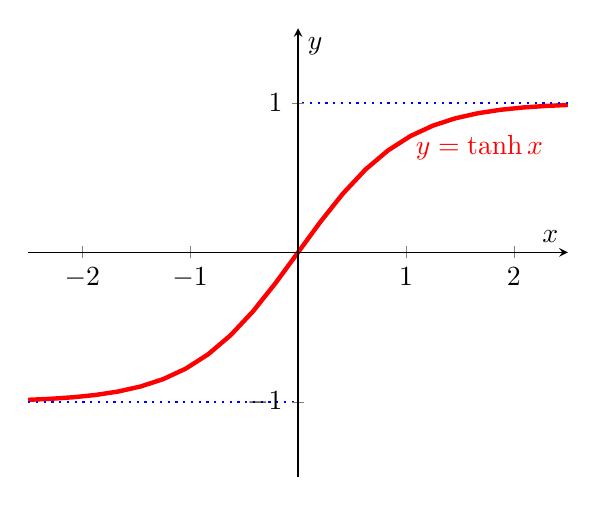
\begin{tikzpicture}
\begin{axis}[
xmin=-2.5, xmax=2.5,
ymin=-1.5, ymax=1.5,
axis lines=center,
axis on top=true,
domain=-2.5:2.5,
ylabel=$y$,
xlabel=$x$,
]
\addplot [mark=none,draw=red,ultra thick] {tanh(\x)};
\node [right, red] at (axis cs: 1,0.7) {$y = \tanh x$};
\draw [blue, dotted, thick] (axis cs:-2.5,-1)-- (axis cs:0,-1);
\draw [blue, dotted, thick] (axis cs:+2.5,+1)-- (axis cs:0,+1);
\end{axis}
\end{tikzpicture}
\item rectified linear unit
\begin{tikzpicture}
\begin{axis}
[xmin=-1.5, xmax=1.5,
ymin=-1.5, ymax=1.5,
axis lines=center,
axis on top=true,
domain=-1.5:1.5,
ylabel=$a$,
xlabel=$z$,]
\draw [purple, thick] (axis cs:-1,0) -- (axis cs:0,0);
\draw [purple, thick] (axis cs:0,0) -- (axis cs:1,1);
\node [right, purle] at (axis cs: 0.3,0.7) {$a = max(0,z)$};
\end{axis}
\end{tikzpicture}
\item Leaky ReLU
\begin{tikzpicture}
\begin{axis}
[xmin=-1.5, xmax=1.5,
ymin=-1.5, ymax=1.5,
axis lines=center,
axis on top=true,
domain=-1.5:1.5,p
ylabel=$a$,
xlabel=$z$,]
\draw [purple, thick] (axis cs:-1,-0.2) -- (axis cs:0,0);
\draw [purple, thick] (axis cs:0,0) -- (axis cs:1,1);
\node [right, purle] at (axis cs: 0.3,0.7) {$Leaky ReLU$};
\end{axis}
\end{tikzpicture}
\item sigmoid function: never use except for output
\item tanh is better
\item ReLU: commonly used
\end{itemize}
\subsection{Random initialization}
\label{sec-2-3}
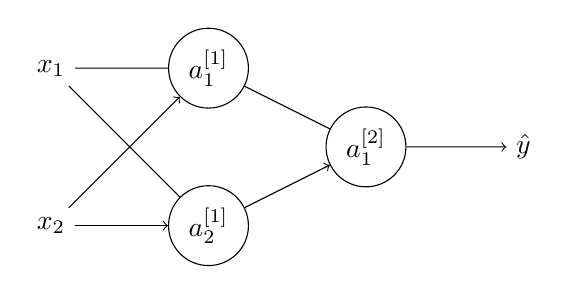
\begin{tikzpicture}
\node (x1) at (0,2) {$x_1$};
\node (x2) at (0,0) {$x_2$};
\node (a1) at (2,2) [circle,draw] {$a_1^{[1]}$};
\node (a2) at (2,0) [circle,draw] {$a_2^{[1]}$};
\node (a12) at (4,1) [circle,draw] {$a_1^{[2]}$};
\node (y) at (6,1) {$\hat{y}$};
\draw [->] (x1) -- (a1) -- (a12) -- (y);
\draw [->] (x1) -- (a2) -- (a12);
\draw [->] (x2) -- (a1);
\draw [->] (x2) -- (a2);
\end{tikzpicture}
if w is 0
$a_1^{[1]}$ will be the same as $a_2^{[1]}$
\section{Week3}
\label{sec-3}
\subsection{Deep neural network notation}
\label{sec-3-1}
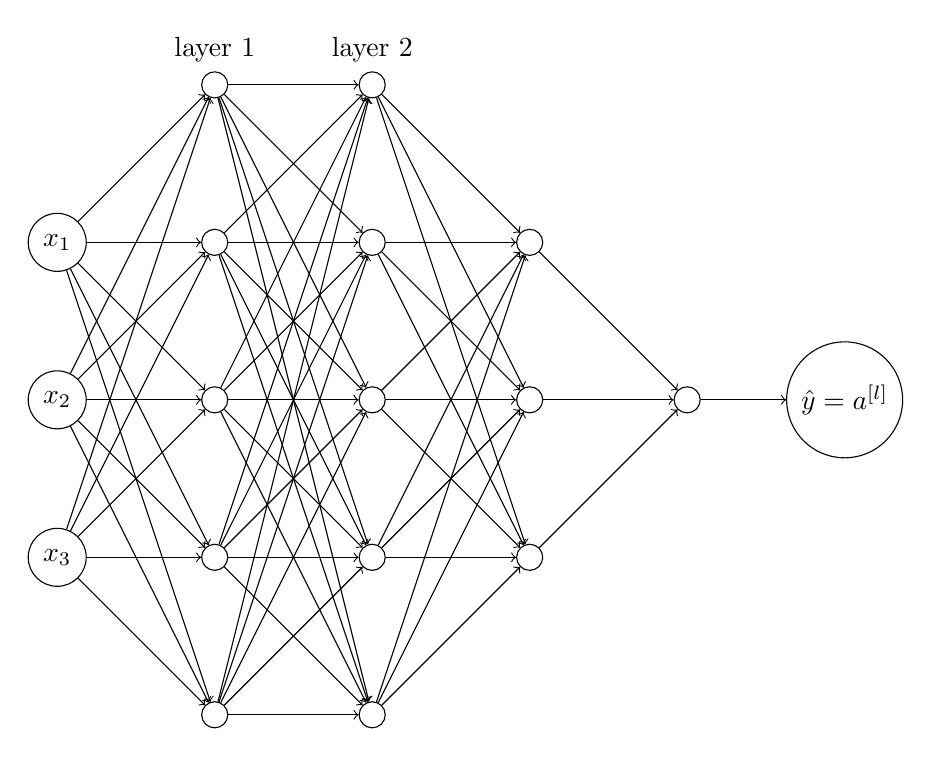
\begin{tikzpicture}
\node (x1) at (0, 6) [circle, draw] {$x_1$};
\node (x2) at (0, 4) [circle, draw] {$x_2$};
\node (x3) at (0, 2) [circle, draw] {$x_3$};
\node (n11) at (2, 8) [circle, draw, label=above:layer 1] {};
\node (n12) at (2, 6) [circle, draw] {};
\node (n13) at (2, 4) [circle, draw] {};
\node (n14) at (2, 2) [circle, draw] {};
\node (n15) at (2, 0) [circle, draw] {};
\node (n21) at (4, 8) [circle, draw, label=above:layer 2] {};
\node (n22) at (4, 6) [circle, draw] {};
\node (n23) at (4, 4) [circle, draw] {};
\node (n24) at (4, 2) [circle, draw] {};
\node (n25) at (4, 0) [circle, draw] {};
\node (n31) at (6, 6) [circle, draw] {};
\node (n32) at (6, 4) [circle, draw] {};
\node (n33) at (6, 2) [circle, draw] {};
\node (n41) at (8, 4) [circle, draw] {};
\node (y) at (10, 4) [circle, draw] {$\hat{y}=a^{[l]}$};
\draw [->] (x1) -- (n11);
\draw [->] (x1) -- (n12);
\draw [->] (x1) -- (n13);
\draw [->] (x1) -- (n14);
\draw [->] (x1) -- (n15);
\draw [->] (x2) -- (n11);
\draw [->] (x2) -- (n12);
\draw [->] (x2) -- (n13);
\draw [->] (x2) -- (n14);
\draw [->] (x2) -- (n15);
\draw [->] (x3) -- (n11);
\draw [->] (x3) -- (n12);
\draw [->] (x3) -- (n13);
\draw [->] (x3) -- (n14);
\draw [->] (x3) -- (n15);
\draw [->] (n11) -- (n21);
\draw [->] (n11) -- (n22);
\draw [->] (n11) -- (n23);
\draw [->] (n11) -- (n24);
\draw [->] (n11) -- (n25);
\draw [->] (n12) -- (n21);
\draw [->] (n12) -- (n22);
\draw [->] (n12) -- (n23);
\draw [->] (n12) -- (n24);
\draw [->] (n12) -- (n25);
\draw [->] (n13) -- (n21);
\draw [->] (n13) -- (n22);
\draw [->] (n13) -- (n23);
\draw [->] (n13) -- (n24);
\draw [->] (n13) -- (n25);
\draw [->] (n14) -- (n21);
\draw [->] (n14) -- (n22);
\draw [->] (n14) -- (n23);
\draw [->] (n14) -- (n24);
\draw [->] (n14) -- (n25);
\draw [->] (n15) -- (n21);
\draw [->] (n15) -- (n22);
\draw [->] (n15) -- (n23);
\draw [->] (n15) -- (n24);
\draw [->] (n15) -- (n25);
\draw [->] (n21) -- (n31);
\draw [->] (n21) -- (n32);
\draw [->] (n21) -- (n33);
\draw [->] (n22) -- (n31);
\draw [->] (n22) -- (n32);
\draw [->] (n22) -- (n33);
\draw [->] (n23) -- (n31);
\draw [->] (n23) -- (n32);
\draw [->] (n23) -- (n33);
\draw [->] (n24) -- (n31);
\draw [->] (n24) -- (n32);
\draw [->] (n24) -- (n33);
\draw [->] (n25) -- (n31);
\draw [->] (n25) -- (n32);
\draw [->] (n25) -- (n33);
\draw [->] (n31) -- (n41);
\draw [->] (n32) -- (n41);
\draw [->] (n33) -- (n41);
\draw [->] (n41) -- (y);
\end{tikzpicture}
$l$ is the \$l\$th layer
$n^{[l]}=\#units$ in layer $l$
$a^{[l]}=g^{[l]}(z^{[l]})$ is activations in l
\subsection{Circuit theory and deep learning}
\label{sec-3-2}
Informally: There are functions you can compute with a "small"
L-layer deep neural network that shallower networks require exponentially
more hidden units to compute
\section{Week4}
\label{sec-4}
\subsection{Bias and variance}
\label{sec-4-1}

\begin{center}
\begin{tabular}{lllll}
\hline
Train set error & 1\% & 15\% & 15\% & 1\%\\
Dev set error & 11\% & 16\% & 30\% & 0.5\%\\
 & high variance & high bias & high bias and variance & low\\
 &  &  &  & \\
\hline
\end{tabular}
\end{center}
\subsection{Basic recipe for machine learning}
\label{sec-4-2}
   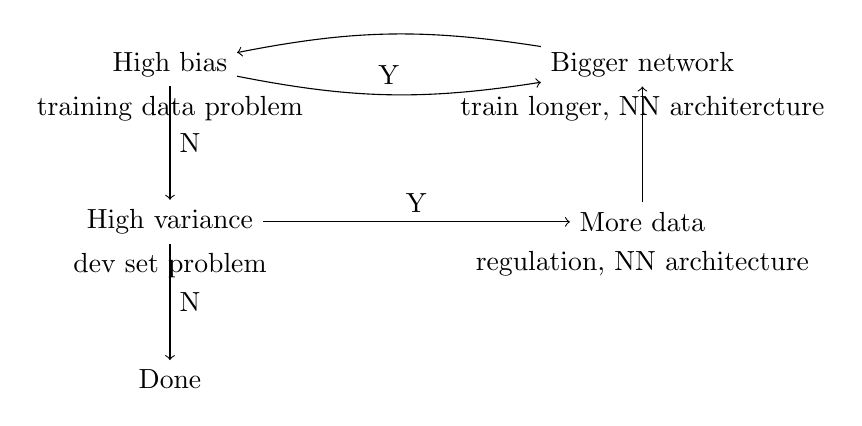
\begin{tikzpicture}[auto]
\node (x11) at (0,0)  {Done};
\node (x12) at (0,2) [label=below:dev set problem] {High variance};
\node (x13) at (0,4) [label=below:training data problem] {High bias};
\node (x22) at (6,2) [label=below:{regulation, NN architecture}] {More data};
\node (x23) at (6,4) [label=below:{train longer, NN architercture}] {Bigger network};
\draw [->] (x13) to [bend right = 10] node {Y}  (x23);
\draw [<-] (x13) to [bend left = 10] (x23);
\draw [->] (x13) to node {N} (x12);
\draw [->] (x12) to node {N} (x11);
\draw [->] (x12) to node {Y} (x22);
\draw [->] (x22) to (x23);
\end{tikzpicture}
\subsection{Regularization}
\label{sec-4-3}
\begin{description}
\item[{L2 regulation--logistic regression}] $\mathcal{J}(w,b)=\frac{1}{m}\displaystyle\sum_{i=1}^m\mathcal{L}(\hat{y}^{(i)}
        ,y^{(i)})+\frac{\lambda}{2m}||w||_2^2$
        $\lambda$ is regulazation parameter
\item[{neural network}] \begin{itemize}
\item $\mathcal{J}(w^{[1]},b^{[1]},\dots,w^{[L]},b^{[L]})=\frac{1}{m}\displaystyle\sum_{i=1}^m
       \mathcal{L}(\hat{y}^{(i)},y^{(i)})+\frac{\lambda}{2m}||w^{[l]}||_F^2$
\item[{Frobenius norm}] \begin{itemize}
\item $||w^{[l]}||^2=\displaystyle\sum_{i=1}^{n^{[l-1]}}\sum_{j=1}^{n^{[l]}}
         (w_{ij}^{[l]})^2$
\item $dw^{[l]}=\dots + \frac{\lambda}{m}w^{[l]}$
\end{itemize}
\end{itemize}
\item[{Why regulazation}] \begin{itemize}
\item If we set $\lambda\to$ big enough, the frobenius norm may tend to approach to 0, which
will make some $w^{[l]}$ to be 0 as if hidden layer become just logistic
regression, thus overfit may change to just right or high bias.
\item If we use $tanh$ as activation function, $\lambda\uparrow$, $w^{[l]}\downarrow$,$z^{[l]}=w^{[l]}a^{[l-1]}+b^{[l]}\downarrow$,
notice in $tanh$, when $z\to 0$, it tends to be linear function, thus handle
the overfitting problem
\end{itemize}
\item[{dropout regulation}]
\end{description}
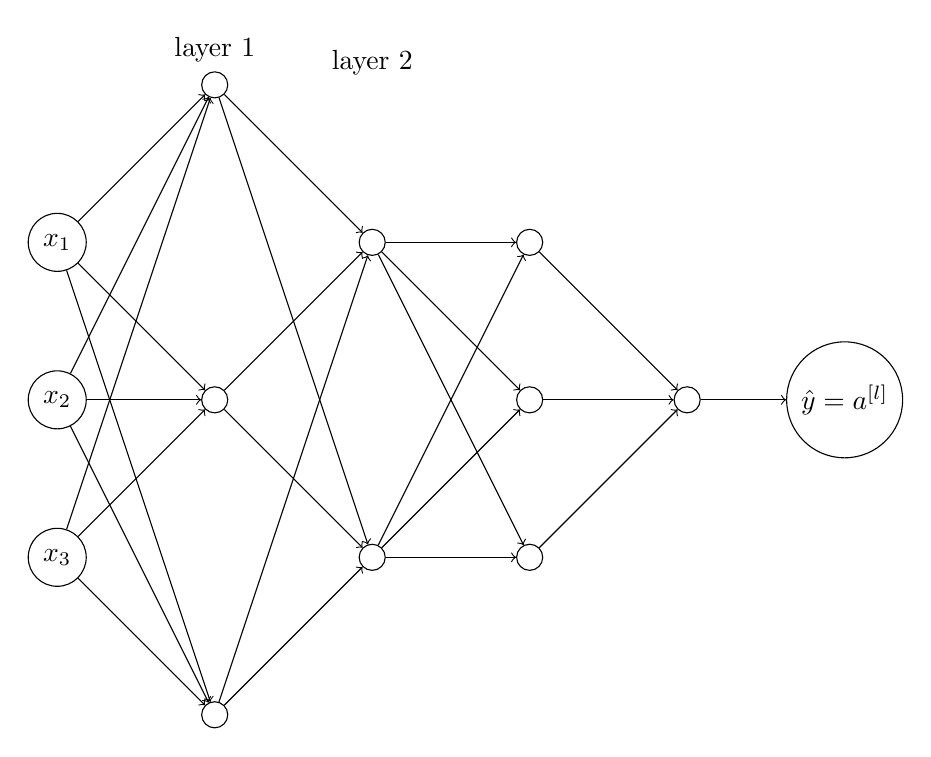
\begin{tikzpicture}
[cross/.style={cross out, draw=black, minimum size=2*(#1-\pgflinewidth), inner sep=0pt, outer sep=0pt}]

\node (x1) at (0, 6) [circle, draw] {$x_1$};
\node (x2) at (0, 4) [circle, draw] {$x_2$};
\node (x3) at (0, 2) [circle, draw] {$x_3$};
\node (n11) at (2, 8) [circle, draw, label=above:layer 1] {};
\node (n12) at (2, 6) [circle, draw,cross] {};
\node (n13) at (2, 4) [circle, draw] {};
\node (n14) at (2, 2) [circle, cross] {};
\node (n15) at (2, 0) [circle, draw] {};
\node (n21) at (4, 8) [circle, draw, label=above:layer 2, cross] {};
\node (n22) at (4, 6) [circle, draw] {};
\node (n23) at (4, 4) [circle, draw, cross] {};
\node (n24) at (4, 2) [circle, draw] {};
\node (n25) at (4, 0) [circle, draw, cross] {};
\node (n31) at (6, 6) [circle, draw] {};
\node (n32) at (6, 4) [circle, draw] {};
\node (n33) at (6, 2) [circle, draw] {};
\node (n41) at (8, 4) [circle, draw] {};
\node (y) at (10, 4) [circle, draw] {$\hat{y}=a^{[l]}$};
\draw [->] (x1) -- (n11);
\draw [->] (x1) -- (n13);
\draw [->] (x1) -- (n15);
\draw [->] (x2) -- (n11);
\draw [->] (x2) -- (n13);
\draw [->] (x2) -- (n15);
\draw [->] (x3) -- (n11);
\draw [->] (x3) -- (n13);
\draw [->] (x3) -- (n15);
\draw [->] (n11) -- (n22);
\draw [->] (n11) -- (n24);
\draw [->] (n13) -- (n22);
\draw [->] (n13) -- (n24);
\draw [->] (n15) -- (n22);
\draw [->] (n15) -- (n24);
\draw [->] (n22) -- (n31);
\draw [->] (n22) -- (n32);
\draw [->] (n22) -- (n33);
\draw [->] (n24) -- (n31);
\draw [->] (n24) -- (n32);
\draw [->] (n24) -- (n33);
\draw [->] (n31) -- (n41);
\draw [->] (n32) -- (n41);
\draw [->] (n33) -- (n41);
\draw [->] (n41) -- (y);
\end{tikzpicture}

\begin{description}
\item[{implementing dropout}]
\item[{Intuition}] \begin{itemize}
\item Can't rely on any one feature, so have to spread out weights since they can go
away randomly
\end{itemize}
\item[{other methods}] \begin{itemize}
\item data augmentation
i.e. picture : flip, rotate
\item early stopping
\end{itemize}
\end{description}
\subsection{Setting up your optimization problem}
\label{sec-4-4}
\begin{itemize}
\item normalizing inputs
\item vanishing / exploding gradients
\item Weight initialization for deep networks
\begin{verbatim}
W[l] = np.random.rand(shape) * np.sqrt(1 / n[l - 1])
\end{verbatim}
\item Gradient check for a neural network
Take $W^{[1]}, b^{[1]},\dots,W^{[L]},b^{[L]}$ and reshape into a big vector $\theta$
$\mathcal{J}(W^{[1]}, b^{[1]},\dots,W^{[L]},b^{[L]})=\mathcal{J}(\theta)$
Take $dW^{[1]}, db^{[1]},\dots,dW^{[L]},db^{[L]}$ into $d\theta$
Now does $d\theta$ is the gradient of $\mathcal{J}(\theta)$
\begin{itemize}
\item for each i
$d\theta_{approx}[i]=\frac{\mathcal{J}(\theta_1,\dots,\theta_i+\epsilon,\dots)-
       \mathcal{J}(\theta_1,\dots,\theta_i+\epsilon,\dots)}{2\epsilon}\approx\theta[i]$
\item Check
$\frac{||d\theta_{approx}-d\theta||_2}{||d\theta_{approx}||_2-||d\theta||_2}$
\item don't use in training -- only in debug
\end{itemize}
\end{itemize}
% Emacs 25.2.1 (Org mode 8.2.10)
\end{document}
